%!Tex Ts-program = xelatex
%!figpath = .
\documentclass[11pt,openany]{book}              % Book class in 11 points

%\documentclass[justified,twoside]{tufte-book}
%\usepackage[UTF8]{ctex}


\parindent0pt  \parskip10pt             % make block paragraphs
%\raggedright                            % do not right justify
\usepackage{xcolor}
\usepackage{amsmath}
\usepackage{amssymb}
\usepackage{bm}
\usepackage[round]{natbib}
\usepackage{graphicx}
\usepackage{subfigure}
\usepackage{amsthm}
\usepackage{tgpagella}
\usepackage{enumerate}
\usepackage{emptypage}
\usepackage{multirow}
\usepackage{booktabs}
\usepackage{braket}
\usepackage[LGR,T1]{fontenc}
\newcommand{\textgreek}[1]{\begingroup\fontencoding{LGR}\selectfont#1\endgroup}
\usepackage{lipsum}
\usepackage{tcolorbox}


\usepackage{microtype}


\definecolor{echodrk}{HTML}{0099cc}
\definecolor{mymauve}{rgb}{0.58,0,0.82}
\usepackage[colorlinks,linkcolor=mymauve,citecolor=echodrk]{hyperref}
\usepackage{cleveref}
\usepackage{pgfplots}

\definecolor{boxgray}{rgb}{0.9,0.9,0.9}
\definecolor{boxpink}{rgb}{0.9,0.7,0.7}

\renewcommand\vec{\mathbf}
\newcommand\mat{\mathbf}

\makeatletter
\renewcommand{\thesection}{%
  \ifnum\c@chapter<1 \@arabic\c@section
  \else \thechapter.\@arabic\c@section
  \fi
}
\makeatother



\usepackage{marginnote}
\renewcommand*{\marginfont}{\footnotesize}
\newcommand{\joan}[1]{{\color{green}#1}}
\newcommand{\michael}[1]{{\color{magenta}#1}} \newcommand{\taco}[1]{{\color{blue}#1}}
\newcommand{\petar}[1]{{\color{cyan}#1}}


\definecolor{olivegreen}{HTML}{006400}
\definecolor{echoblue}{HTML}{0099CC}
\definecolor{gold}{HTML}{F09A00}
\definecolor{vividred}{HTML}{E60B42}
\definecolor{echonavy}{HTML}{0054B2}
\definecolor{darkgry}{HTML}{333333}
\definecolor{echopurple}{HTML}{9400D1}
\usepackage{tikz}
\tikzset{every picture/.style={line width=0.75pt}} %set default line width to 0.75pt    


\newcommand*{\horzbar}{\rule[.5ex]{2.5ex}{0.5pt}}


\newtheoremstyle{break}
{\topsep}{\topsep}%
{\itshape}{}%
{\bfseries}{}%
{\newline}{}%
%\theoremstyle{break}

\newtheorem{definition}{Definition}
\newtheorem{theorem}{Theorem}
\newtheorem{remark}{Remark}
\newtheorem{example}{Example}
\newtheorem{corollary}{Corollary}
\newtheorem{consequence}{Consequence}
\newtheorem{conjecture}{Conjecture}
\newtheorem{problem}{Problem}
\newtheorem{solution}{Solution}
\newcommand{\sign}{{\rm sign}}
\newcommand{\argmin}{\mathop{\rm argmin}}
\newcommand{\argmax}{\mathop{\rm argmax}}
\newcommand{\tr}{\mathop{\rm tr}}
\newcommand{\dd}{{\rm d}}

\usepackage{fancyhdr}

\fancypagestyle{plain}{ %
  \fancyhf{} % remove everything
  \renewcommand{\headrulewidth}{0pt} % remove lines as well
  \renewcommand{\footrulewidth}{0pt}
}


\fancypagestyle{fancybook}{%
  \fancyhf{}%
  % Note the ## here. It's required because \fancypagestyle is making a macro (\ps@fancybook).
  % If we just wrote #1, TeX would think that it's the argument to \ps@fancybook, but
  % \ps@fancybook doesn't take any arguments, so TeX would complain with an error message.
  % You are not expected to understand this.
  \renewcommand*{\sectionmark}[1]{ \markright{\thesection\ ##1} }%
  %\renewcommand*{\chaptermark}[1]{ \markboth{\chaptername\ \thechapter: ##1}{} }%
  % Increase the length of the header such that the folios 
  % (typography jargon for page numbers) move into the margin
  \fancyhfoffset[LE]{6mm}% slightly less than 0.25in
  \fancyhfoffset[RO]{6mm}%
  % Put some space and a vertical bar between the folio and the rest of the header
  \fancyhead[LE]{\thepage\hskip3mm\vrule\hskip3mm}%
  \fancyhead[RO]{\rightmark\hskip3mm\vrule\hskip3mm\thepage}%
}
\pagestyle{fancybook}

%\usepackage{appendix}

\usepackage[titletoc]{appendix}


%\fancyhf[HLE,HRO]{Bruna et al.}
\pagestyle{empty}

\newcommand{\rarr}{\rightarrow}

\begin{document}
\chapter*{Some Property of Ising Model}
\vspace{-1cm}
{\fontsize{18.0pt}{\baselineskip}\selectfont  Yongle Bai 202011150087}

\section{The detailed setup of the problem}
The Ising model (or Lenz-Ising model or Ising-Lenz model), named after the physicists Ernst Ising and Wilhelm Lenz, is a mathematical model of ferromagnetism in statistical mechanics.
The model consists of discrete variables that represent magnetic dipole moments of atomic "spins" that can be in one of two states (+1 or −1).
The spins are arranged in a graph, usually a lattice (where the local structure repeats periodically in all directions), allowing each spin to interact with its neighbors.
Neighboring spins that agree have a lower energy than those that disagree; the system tends to the lowest energy but heat disturbs this tendency, thus creating the possibility of different structural phases.
The model allows the identification of phase transitions as a simplified model of reality.
The two-dimensional square-lattice Ising model is one of the simplest statistical models to show a phase transition.

Now we consider a \(2\)-dimensional lattice with period boundary and size \(n \times n\).
We use \(\Lambda:=\mathbb{Z}_n \times \mathbb{Z}_n\) as the index set.
Let \(\sigma=\{ \sigma_k\}_{k \in \Lambda}\) be the state of the lattice.
The direction of each spin in the lattice is regarded as an element in \(\sigma\), and \(\pm 1\) represent two direction.
For any two adjacent sites \(i,j\in \Lambda \) there is an spin-spin interaction \(J\).
Also a site \(j\in \Lambda \) has an external magnetic field \(H\) interacting with it. The energy of a configuration \(\sigma\) is given by the Hamiltonian function
\begin{equation}\label{equ:1}
	H(\sigma)=-\sum_{i,j\in\Lambda,i \sim j} J \sigma_i \sigma_j-\sum_{i \in \Lambda}H \sigma_i
\end{equation}
where \(i \sim j\) means \(i\) and \(j\) is adjacent.
The configuration probability is given by the Boltzmann distribution with inverse temperature \( \beta \geq 0\):

\[ \mathbb{P}(\sigma )={\frac {e^{-\beta H(\sigma )}}{Z}},\]

where \( \beta =1/(k_{B}T)\), and the normalization constant

\[ Z=\sum _{\sigma }e^{-\beta H(\sigma )}\]

is the partition function.

Our aim is to find out how does the temperature influence the property of lattice and determine the critical temperature.
In this article, we will use Metropolis sampling to solve following two problem:

\begin{problem}\label{pro:1}
Take \(J=1, k_B=1, H=0\), let \(N\) be the size of the lattice and \(T\) be the temperature.
Caculate internal energy \(u\) in the process:
\begin{equation}
	u=\frac{U}{N^2},U=\mathbb{E}(H)=\sum_{\sigma\in 2^\Lambda}\mathbb{P}(\sigma)H( \sigma)
\end{equation}
and specific heat \(c\):
\begin{equation}
	c=\frac{C}{N^2}, C=\frac{k_B}{T^2}\mathbb{V}\mathrm{ar}(H)=\frac{k_B}{T^2}( \mathbb{E}( H^2)-\mathbb{E}( H)^2)
\end{equation}
where \(\mathbb{V}\mathrm{ar}\) is the variance.
And plot graph of \(u-T, c-T\).
And check the temperature near the critical temperature \(T_c = \frac{2| J|}{k_B \ln ( 1+\sqrt{2})}\).

\end{problem}
\begin{problem}\label{pro:2}
Take \(J=1, k_B=1\), \(H \neq 0\). Fixing \(T, H\),
Caculate magnetization \(m\) in the process:
\begin{equation}
	m=\frac{M}{N^2}, M=\mathbb{E}(\sum_{i \in \Lambda} \sigma_i ).
\end{equation}
And plot graph of \(m-(T, H)\). You may find some interesting result near \(T = T_c\).

\end{problem}

\section{The procedure you take to do the computation }
Whether to accept the convert of a spin is deicided by the change of Hamiltonian before and after the convert, write \(\Delta H\), and temperature \(T\).
If \(\Delta H<0\), then accept the convert.
If \(\Delta H > 0 \), then we accept the convert with probabilty of \(\mathrm{e}^{\frac{- \Delta H}{\beta}}\).
After the convert of the spin, a convert will happen afterwards.
The procedure of the computation is following:
\begin{enumerate}
	\item First of all, set the initial paraments: Set up the grid to imitate the magnet.
	      Choose a state \(X_1\) randomly in \(2^\Lambda\).
	\item Secondly, we randomly choose a point in \(X_n\) to try to change its direction of magnet, and caculate the changed energy \(\Delta H\).
	      And then, judge whether to accept the direction change of this point.
	      If accepted, then the point will change direction; else, it will remain the old direction. Then we get \(X_{n+1}\).
	\item Repeat the process above for a long time, write \(Y\).
	\item Use \(\mathbb{E}'( f):=\sum_{t=X}^{Y} f( X_t)\) to estimate \(\mathbb{E}( f)\), to caculate \(c,u\) and \(m\), where \(X\) is a certain number choosed between \(0\) and \(Y\).
	\item Last, plot the graphs and analysis the results.
\end{enumerate}




\section{Analysis of the numerical results }
\begin{solution}
	In \Cref{pro:1}, we let \(T\) ranges in \(0.5\sim 4\) and convert \(1000000\) steps.
	In \Cref{fig:Tu} we can see as temperature become higher and higher, the value of the average Hamiltonian, \(u\), become bigger and bigger.
	That's means high temperature will supply more energy for the spins to get a state with high Hamiltonian.
	More over, we can find that the growth rate of \(u\) is highest near \(T=T_c\).
	When \(T\) is far from \(T_c\), the value of \(u\) is a virtual constant.
	\begin{figure}\label{fig:Tu}
		\centering
		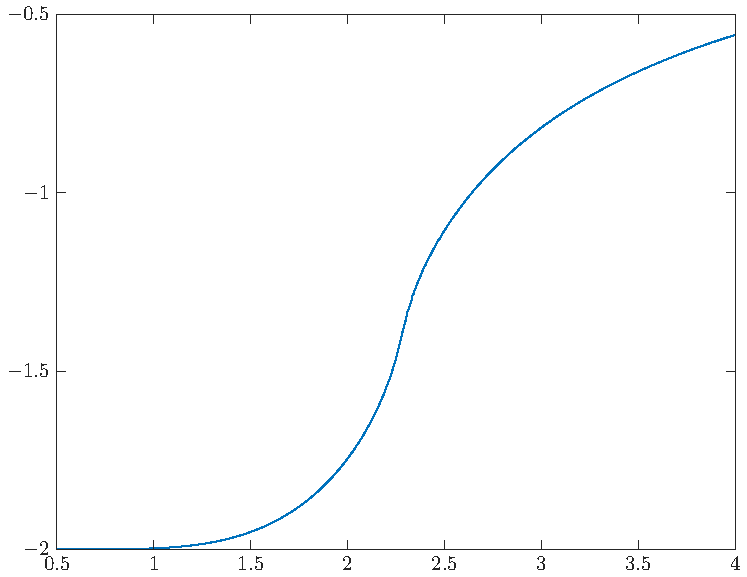
\includegraphics[width=0.8\linewidth]{Tu.pdf}
		\caption{T-u}
	\end{figure}
	In \Cref{fig:Tc} we can see the more temperature \(T\) go near \(T_c\), the higher the critical

	\begin{figure}\label{fig:Tc}
		\centering
		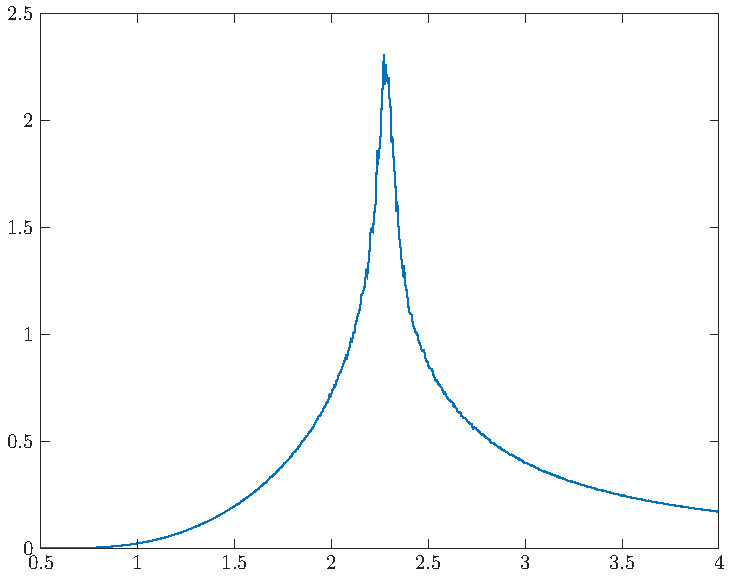
\includegraphics[width=0.8\linewidth]{Tc.pdf}
		\caption{T-c}
	\end{figure}
	\begin{figure}\label{fig:THM}
		\centering
		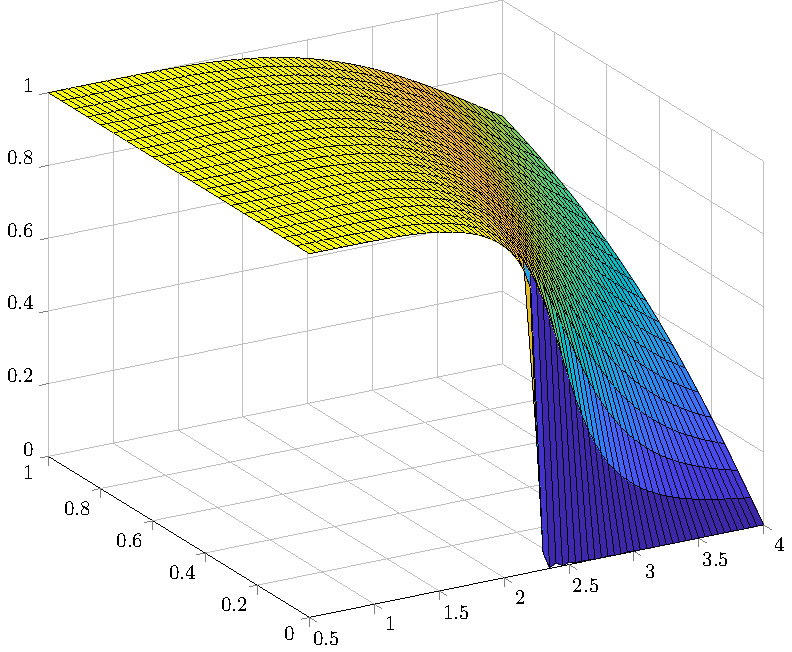
\includegraphics[width=0.8\linewidth]{THM.pdf}
		\caption{T-H-m}
	\end{figure}




\end{solution}

\section{The issues you encounter and how you overcome }
First of all, when we was running our program, our compute is not capable enough. But fortunately,
we have a generous teacher, who borrowed us his compute to complete our program.

\section{ Possible discussion about the results and further thinking }
Ising model can be applied to many other situations and fields. For example, opinion dynamics.
Consider a group of people, each person can support one of two different candidates (like A and B).
The candidate one support may change after exchanging ideas with sourroundings.
What's more, the residents there may be influenced by advertisement of candidates. This is a typical
reality situation for Ising model.

Besides, we can apply the Ising model to neuroscience. The activity of neuros in the brain can be
modelled statistically. Each neuron at anytime is either active or inactive. Hopfield suggested in 1982
that a dynamic Ising model would provide a first approximate to a neural network which is capable of learning.
And following the general approach of a lot scientists, we can model the process of neurons by the following
model. Given a collection of neurons, we assume the energy as:
\begin{equation}
	\, E = -1/2 \sum_{ij}J_{ij}SiSj-\sum_i h_iS_i
\end{equation}
In this process, we can apply Ising model to simulate it.
%\bibliographystyle{plainnat}
%\bibliography{report}

\end{document}                          % The required last line
